\chapter{Implementation}

This chapter describes details, problems and limitations of the thesis implementation part.

The implementation of the demo-application is divided into three main parts: compression, streaming and rendering.
The compression is implemented as a standalone Java application, which compresses BTFs from the Bonn University \cite{btfBonn}.
It is possible to adapt any other BTF databases for our demo-application by resampling BTFs \cite{resampling}.
For streaming we use  Node.js \cite{nodejs} platform.
To integrate 3D graphics into HTML page we use XML3D \cite{xml3d}.
The overall model of the demo application is depicted in Figure \ref{fig:overview}.

\begin{figure}[h]
 \centering
 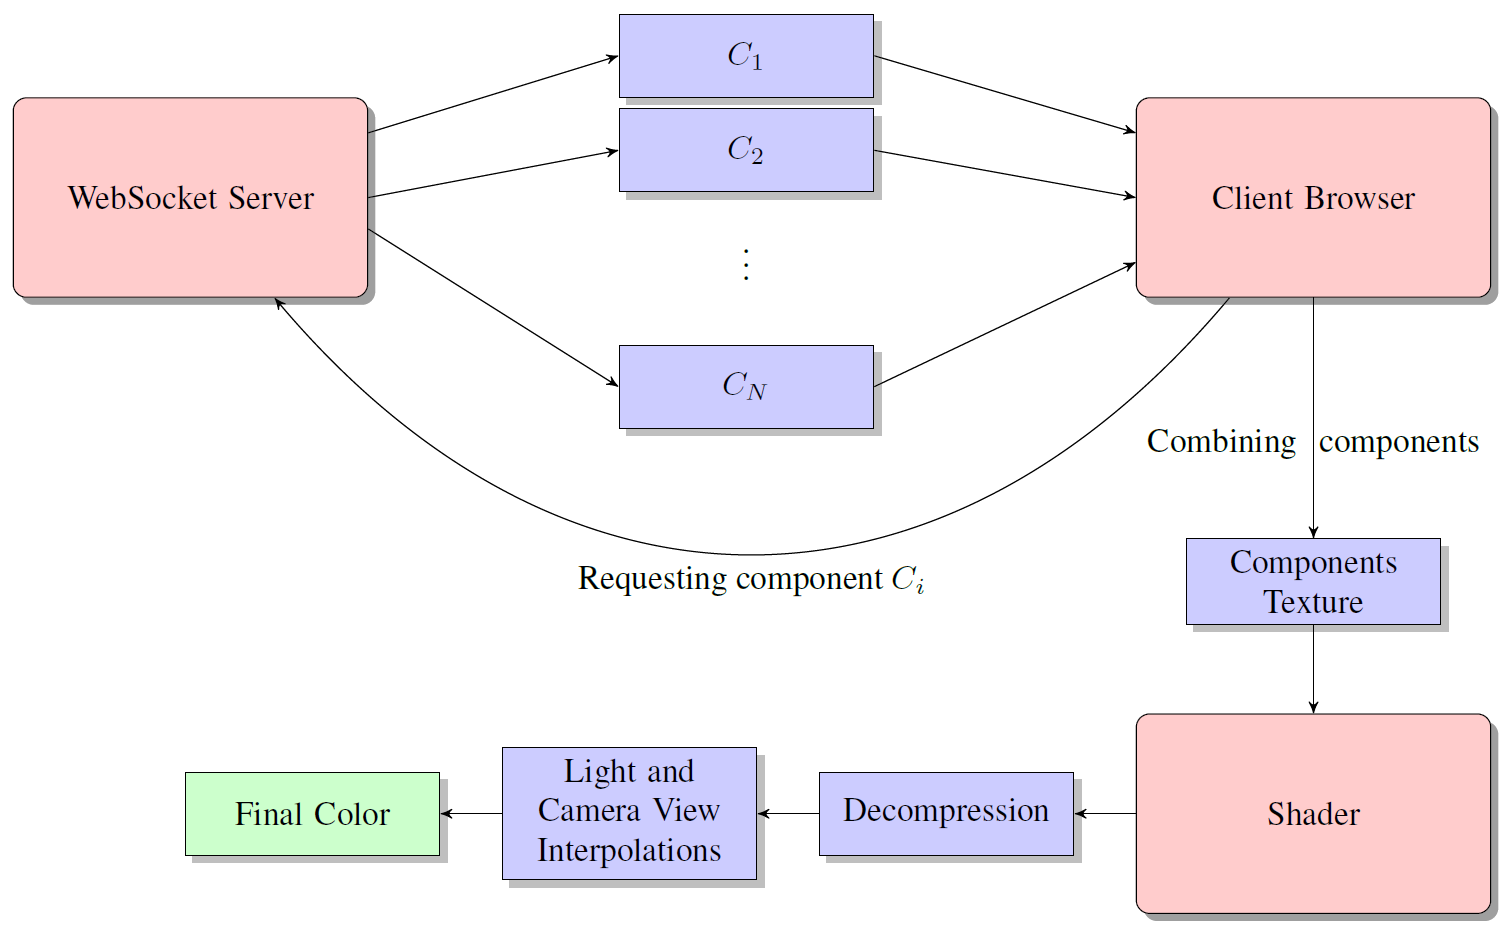
\includegraphics[width=1.0\textwidth]{figures/overview}
 \caption[Model Overview ] {
 	{\bf Model Overview}

	
	}
 \label{fig:overview}
\end{figure}



\section{Compression}
\label{section:impl_compression}

The implementation of the singular value decomposition (SVD) is the main part of the PCA implementation.
 We use \emph{jblas} \cite{jblas} library developed by Mikio Braun. 
 This is a linear algebra library written in Java language, which provides very high performance  \cite{jblas}.
 
The compressed BTFs  have to be sent to the shader. 
  OpenGL Shading Language (GLSL) version 1.0 support uniform arrays, however, they do not fully support dynamic indexing  \cite{glsl}.
Fortunately, it is possible to send arrays of data which are mapped to textures. 
After performing SVD, resulted matrices $U$, $\Sigma$, $V$ are saved as PNG images. (See Chapter \ref{chapter:implementation}).
Values of matrices $U$ and $V$ are in the range of $[-1;1]$.
 Those values have to be mapped to the image domain, i.e. $[0;1]$.
The following function is used to map the values:  

{\centering$f(x)=(x+1)/2$\\}


 Each component of the matrix $U$ is stored as the PNG image.
 For example, if compressed BTF data has $C$ principal components, then this would result in $C$ separate images.
 This is done for streaming purpose, so then principal components can be sent one by one from the server to the client.
 We use  RGBA color space to save four components into the one pixel, because it is possible to do efficient multiplication in the shader by using vector multiplications.
Matrices $V$ and $\Sigma$ are saved in the single shared texture, as they are small in size.

 The matrix $\Sigma$ is a diagonal matrix.
 The values of $\Sigma$ can be bigger than the image color value, i.e. an 8-bit value.
 In practice the values of $\Sigma$ for Bonn University BTFs \cite{btfBonn} are not bigger than four digit number $a_{4}a_{3}a_{2}a_{1}$.
We split the value into two values, i.e. 
 
{\centering$ \underbrace{a_{4}a_{3}}_{R} \underbrace{a_{2}a_{1}}_{G}$\\}
 
It means that two values of $\Sigma$ are mapped into the one pixel, i.e.  one value to RG  channels and the second to BA channels.
If the value of  $\Sigma$ exceed the four digit number, then it is possible to adapt this technique further in the similar manner.


We noticed that in case of Bonn Database \cite{btfBonn} the \emph{jblas} \cite{jblas} library produces relatively sparse values for $U$ and $V$, i.e. close to the zero.
 We scale the data to improve the floating point error caused by mapping of $U$ and $V$ back-and-forth.
The scaling improved the overall decompression error approximately by $5\%$.
 Using the following function we find the scaling factor:
 
 {\centering$ factor(M)=10^{floor(min[log10(min(M)),log10(max(M)]))}$ \\}
 
 where M is the matrix $U$ or $V$. The term $floor(min[log10(min(M)),log10(max(M))])$ calculates the degree with which it is possible to multiply the matrix and preserve the original values range, i.e. $[-1;1]$.
 If it is not possible, the resulting factor will be $1$.
As the decompression is computed as multiplication of $U\Sigma V$, we have to remain the original decompressed BTF values.
We do this by  multiplying each time $\Sigma$ values by the factor $\tfrac{1}{factor(M)}$ if we scale either $U$ or $V$.


 
\section{Streaming}
\label{section:impl_streaming}


We use Node.js \cite{nodejs} as a server side platform, which enables realtime streaming using WebSockets. On top of that, we use BinaryJS \cite{binaryjs} for the binary streaming.
BinaryJS is a framework that uses WebSockets to stream the binary data to the client from the Node.js server.
The server and the client applications are written in JavaScript.



\begin{figure}[h]
 \centering
 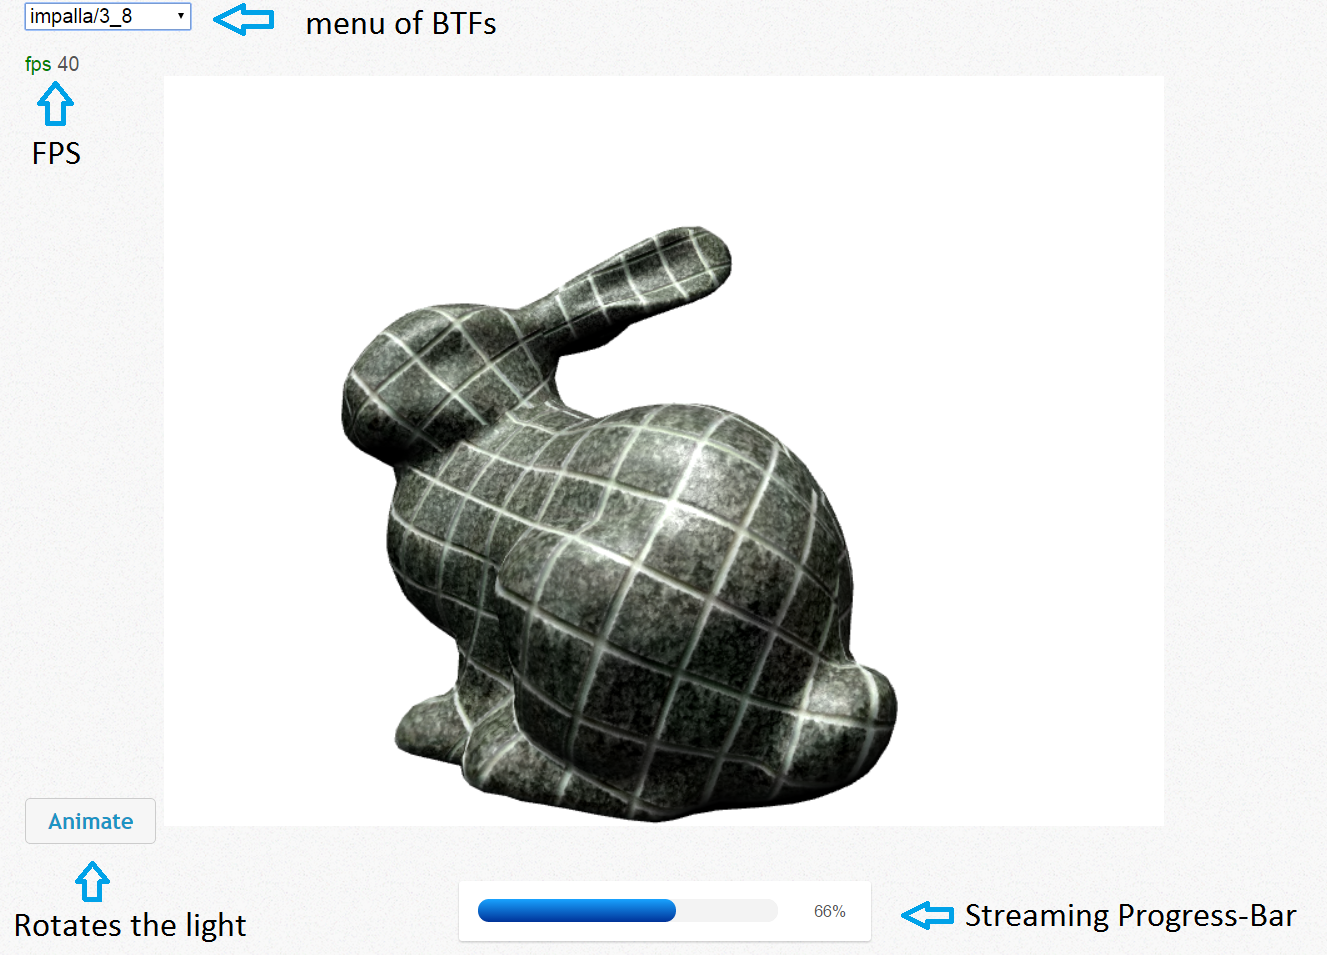
\includegraphics[width=1.0\textwidth]{figures/progress-bar}
 \caption[The streaming progress on the client side] {
 	{\bf The streaming progress on the client side }

 }
 \label{fig:progress-bar}
\end{figure}

We also use Xflow \cite{xflow}, which is a declarative language for data flow processing in realtime.
Xflow is a part of XML3D implementation. We use Xflow for gathering all the transferred principal components and storing them in one common texture $L$. (See Chapter  \ref{section:decompression}).

Consider Figure \ref{fig:streaming} from the Chapter \ref{chapter:streaming} that depicts how the streaming works on practice.
When the user connects to the streaming server and the HTML page loads completely, i.e. all the 3D objects are on the client side, the JavaScript client side sends the message to the Node.js server to start streaming the BTF data.
All the compressed BTFs are located on the Node.js server.
At the start of the stream, we first send texture $R$ and meta data. (See Chapter  \ref{section:decompression}).
Afterwards, each principal component $C_{i}$ are streamed in chunks one by one as PNG images.
Each $C_{i}$ covers all the angular domain, i.e. all the possible camera and light directions.

We decode PNG images using PNG decoder written by Arian Stolwijk \cite{pngreader}. PNG images are decoded to the array of RGB colors and saved to the common texture $L$ in canvas format using Xflow.
Each time the texture $L$ updates the rendering also refreshes.
Even with the first principal component the resulted image looks plausible.
With further components the overall quality of the image improves, i.e. specularities are increasing, small micro-structures become more visible and emphasized.
The user also  able to see the progress-bar of the streaming progress as shown in  Figure \ref{fig:progress-bar}.



Currently the limitation of such streaming approach is the drop of the frame rate when the assembling of the principal components occurs on the client side.
This is caused by the update of the canvas element (texture $L$) each time new component is transmitted to the client.
Also, we did not test the performance of multiple streaming, i.e. if there are several 3D objects that request BTFs at the same time.
 Our current implementation does not support this.
This can be included to the future work. 

\section{Rendering}
\label{section:impl_rendering}


We use XML3D \cite{xml3d} platform to embed 3D graphics into the HTML page. XML3D based on XML and allows for declaring your own 3D scenes and shaders.
XML3D is based on WebGL and JavaScript.

The shader design is depicted in Figure \ref{fig:shader}.
The compressed BTF data comes to the shader in the form of two textures. 
The first texture $L$ stores principal components and the second $R$ stores PCA weights. (See Chapter \ref{section:decompression}).
First, we find three closest directions for the camera and light directions. (See Chapter \ref{chapter:finding_triangle}).
Then, we compute barycentric coordinates for interpolation as described in Chapter \ref{chapter:barycentric}.

\begin{figure}[h]
 \centering
 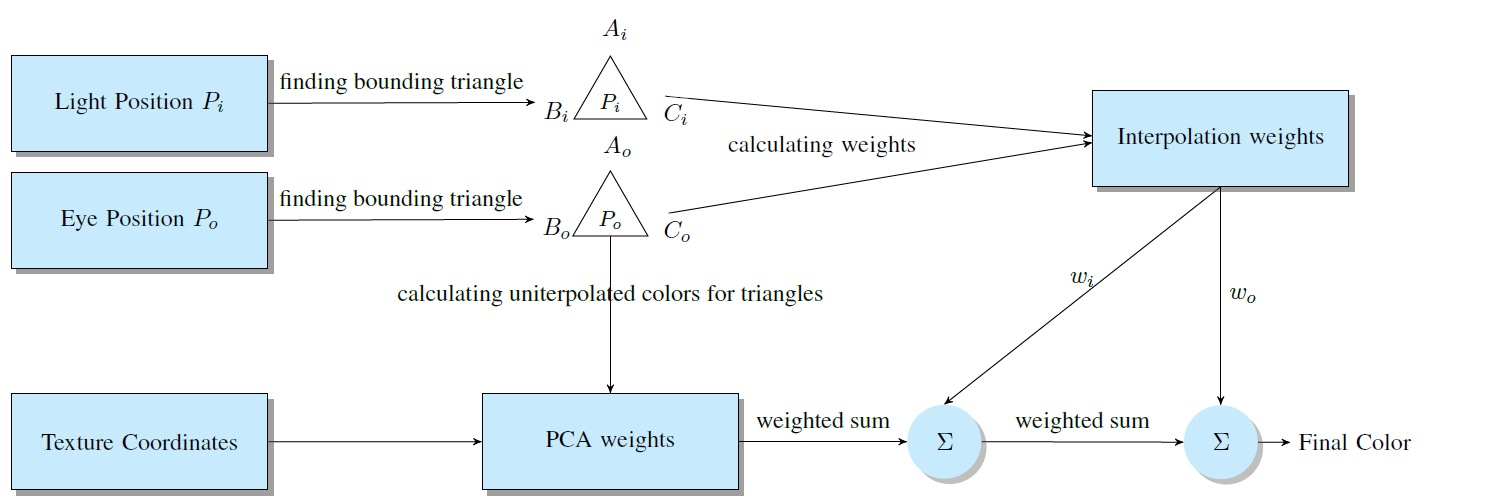
\includegraphics[width=1.0\textwidth]{figures/shader}
 \caption[Shader Design] {
 	{\bf Shader Design }

 }
 \label{fig:shader}
\end{figure}


In the next step we sample the input textures to decompress the needed values for found closest directions.
We have three closest directions per camera and light directions. This means for the interpolation we need to have nine color values. 
For a given texture coordinates $u,v$ we lookup the index of the first principal component, with which it will be possible to start the decompressing.
All the principal components are written linearly in texture $L$, i.e. one by one. 
We have the following mapping to get the needed index:

{\centering$indexL(i,j)= (b*N^2+ (i*N+j))*C$ \\}

where $i=\left \lfloor u*N\right \rfloor$, $j=\left \lfloor v*(N) \right \rfloor$, $b$ is the number of subsets, $N$ is the size of the compressed image and $C$ is number of components.
The parameter $b$ depends on the number of subsets on which PCA is separately done. (See Chapter \ref{section:algorithm_step}).

Texture $R$ stores PCA weights, we lookup the index of suitable compressed image.
The mapping depends on the camera direction $v=(\theta_v,\phi_v)$ and light direction $l=(\theta_l,\phi_l)$.
 It is defined as:

{\centering$ indexR(v,l)=offset(\theta_v,\phi_v)+offset(\theta_l,\phi_l)$\\}

where  $offset(\theta,\phi)=(\tfrac{\theta}{\Delta\theta}+\tfrac{\phi}{\Delta\phi})$, where $\Delta\theta$ and $\Delta\phi$ are quantization step sizes.

When all the indices are computed and textures L and R can be sampled, we decompress the colors as defined in Chapter \ref{section:decompression}.


In a final step we combine nine decompressed colors and early found interpolation weights to get the final color. (See Chapter \ref{chapter:interp_algo}).

The implemented shader has it's own limitations. First of all, the number of principal components has to be fixed for a shader, because GLSL version 1.0 does not allow for dynamic looping \cite{glsl}.
Secondly, the number of principal components are bound by a size of the texture $L$. It means that not all GPUs can handle very big textures. The problem can be fixed by using multiple textures.
But anyway these limitations does not directly influence the performance of the shader, which provides real-time frame rate and performs well even on the mobile devices. (See Figure \ref{fig:progress-bar}).






 



